\documentclass[bluish,slideColor,colorBG,pdf]{prosper}
\hypersetup{pdfpagemode=FullScreen}
\usepackage{graphicx,amsfonts,amsmath}
\def\baselinestretch{1.0}
\setlength{\topmargin}{-60pt}
\setlength{\textheight}{460pt}
\setlength{\oddsidemargin}{0pt}
\setlength{\evensidemargin}{0pt}
\setlength{\textwidth}{660pt}
\setlength{\footskip}{0pt}
\parindent 0.3in
\hyphenpenalty=10000
\tolerance=10000
\pagestyle{empty}

\def\Prob{{\rm Prob\;}}
\def\prob{{\rm \;Prob\;}}
\def\Var{{\rm Var}}        % Var
\def\Cov{{\rm Cov}}        % Cov

\DeclareSymbolFont{AMSb}{U}{msb}{m}{n}
\DeclareMathSymbol{\expect}{\mathalpha}{AMSb}{'105}

\title{Week 6:  Protein sequence models, likelihood, hidden Markov models}
\author{Genome 570}
\institution{February, 2016}

\begin{document}

\maketitle

\begin{slide}[Replace]{Variation of rates of evolution across sites}
\bigskip

The basic way all these models deal with rates of evolution is using the fact
that a rate $\ \mathsf{r}\ $ times as fast is exactly equivalent to evolving
along a branch that is $\ \mathsf{r}\ $ times as long, so that it is easy to
calculate the transition probabilities with rate $\ \mathsf{r}$:

\[
\mathsf{P_{ij}(r,\ t) \ = \ P_{ij}(r\,t)}
\]
\bigskip

The likelihood for a pair of sequences averages over all rates at each
site, using the density function $\ \mathsf{f(r)}\ $ for the distribution of
rates:
\bigskip

{\ptsize{12}
\[
\mathsf{L(t)\ =\ \prod\limits_{i=1}^{\rm sites}\ \left(\int_0^{\infty}\ f(r)\ \pi_{n_i}\;P_{m_in_i}(r\,t)\;dr \right)}
\]
}

\end{slide}

\begin{slide}[Replace]{The Gamma distribution}

\[
\mathsf{f(r)\ =\ \frac{1}{\Gamma(\alpha)\ \beta^\alpha}\;x^{\alpha-1}\;e^{- \frac{x}{\beta}}}
\]

\[
\mathsf{\expect[x]\ =\ \alpha\,\beta}
\]

\[
\mathsf{\Var[x]\ =\  \alpha\,\beta^2}
\]

To get a mean of 1, set  $\mathsf{\beta\ =\ 1/\alpha}$ so that

\[
\mathsf{f(r)\ =\ \frac{\alpha^\alpha}{\Gamma(\alpha) }\ r^{\alpha-1}\ e^{- \alpha r }}.
\]

so that the squared coefficient of variation is $~\mathsf{1/\alpha}$.

\end{slide}

\begin{slide}[Replace]{Gamma distributions}
\bigskip

Here are density functions of Gamma  distributions for three different values
of $\ \mathsf{\alpha}$:

\centerline{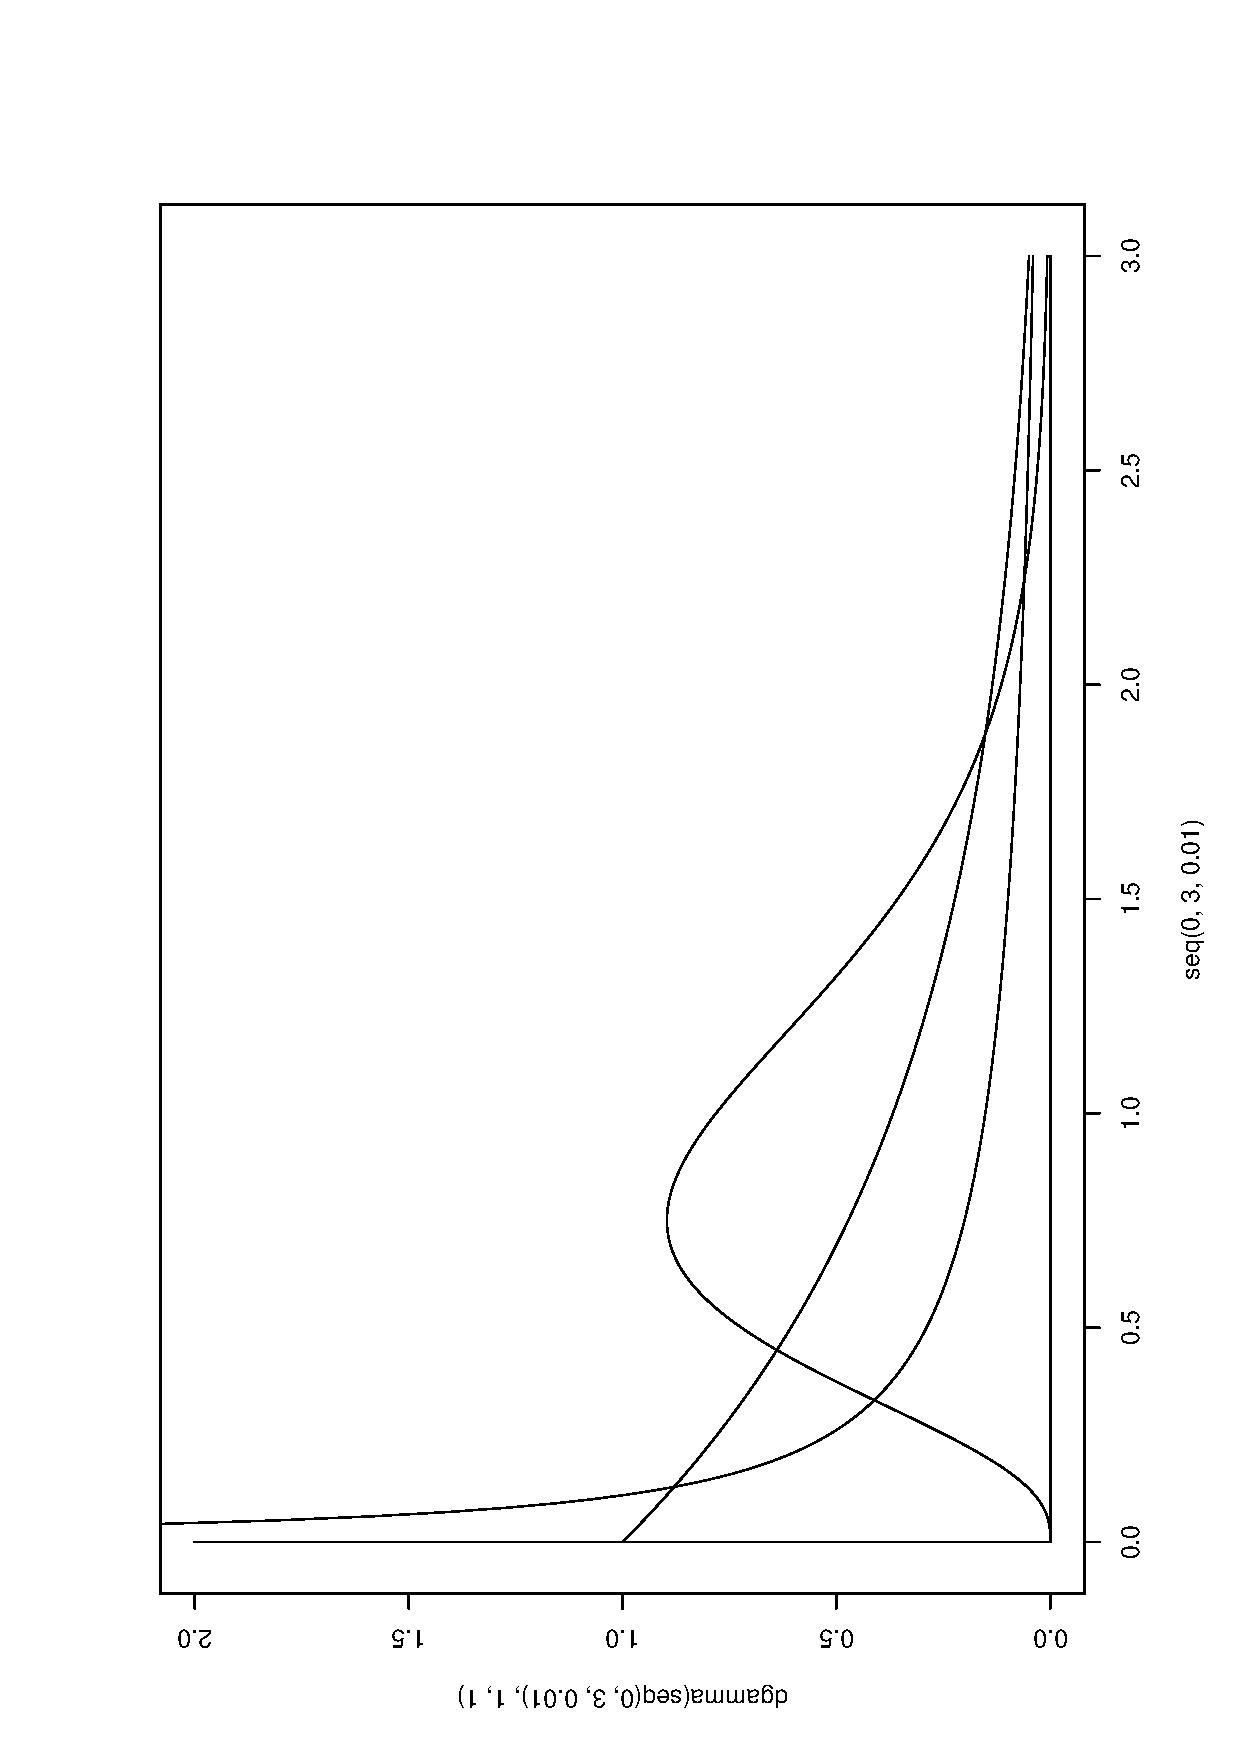
\includegraphics[width=2.9in]{gammadist.idraw}}

\end{slide}

\begin{slide}[Replace]{Gamma rate variation in the Jukes-Cantor model}

For example, for the Jukes-Cantor distance, to get the fraction of sites
different we do

\[
\mathsf{D_S\  =\  \int_0^\infty f(r)\; \frac{3}{4}\left(1-e^{-\frac{4}{3}r\,ut}\right)\;dr}
\]

leading to the formula for $\mathsf{~D~}$ as a function of $\mathsf{~D_S}$

\[
\mathsf{D\ =\ -\frac{3}{4}\; \alpha\ \left[1\ -\ \left(1\ -\ \frac{4}{3}D_S \right)^{-1/\alpha}\ \right]}
\]

\end{slide}

\begin{slide}[Replace]{Gamma rate variation in other models}

For many other distances such as the Tamura-Nei family, the transition probabilites
are of the form

\[
\mathsf{P_{ij}(t)\ =\ A_{ij}\ +\ B_{ij}\;e^{-b t}\ +\ C_{ij}\;e^{-c t}}
\]

and integrating termwise we can make use of the fact that

\[
\mathsf{\expect_r\left[e^{-b\, r\, t} \right]  =  \left(1 + \frac{1}{\alpha}
b\,t \right)^{-\alpha}}
\]
\bigskip

and just use that to replace $\ \mathsf{e^{-bt}}\ $ in the formulas for the
transition probabilities.

\end{slide}

\begin{slide}[Replace]{Dayhoff's PAM001 matrix}

{~~}
\hspace{-0.2in}
{\ptsize{8}  % was: \tiny
\renewcommand{\arraystretch}{0.8}
{~~}\hspace{-0.4in}\begin{tabular}{p{0.01in} p{0.07in} | p{0.10in} p{0.10in} p{0.10in} p{0.10in} p{0.10in} p{0.10in} p{0.10in} p{0.10in} p{0.10in} p{0.10in} p{0.10in} p{0.10in} p{0.10in} p{0.10in} p{0.10in} p{0.10in} p{0.10in} p{0.10in} p{0.10in} p{0.10in}}
 &   & A & R & N & D & C & Q & E & G & H & I & L & K & M & F & P & S & T & W & Y & V\\
&   & ala&arg&asn&asp&cys&gln&glu&gly&his&ile&leu&lys&met&phe&pro&ser&thr&trp&tyr&val\\
\hline
A&ala& 9867& 2& 9& 10& 3& 8& 17& 21& 2& 6& 4& 2& 6& 2& 22& 35& 32& 0& 2& 18\\
R&arg& 1& 9913& 1& 0& 1& 10& 0& 0& 10& 3& 1& 19& 4& 1& 4& 6& 1& 8& 0& 1\\
N&asn& 4& 1& 9822& 36& 0& 4& 6& 6& 21& 3& 1& 13& 0& 1& 2& 20& 9& 1& 4& 1\\
D&asp& 6& 0& 42& 9859& 0& 6& 53& 6& 4& 1& 0& 3& 0& 0& 1& 5& 3& 0& 0& 1\\
C&cys& 1& 1& 0& 0& 9973& 0& 0& 0& 1& 1& 0& 0& 0& 0& 1& 5& 1& 0& 3& 2\\
Q&gln& 3& 9& 4& 5& 0& 9876& 27& 1& 23& 1& 3& 6& 4& 0& 6& 2& 2& 0& 0& 1\\
E&glu& 10& 0& 7& 56& 0& 35& 9865& 4& 2& 3& 1& 4& 1& 0& 3& 4& 2& 0& 1& 2\\
G&gly& 21& 1& 12& 11& 1& 3& 7& 9935& 1& 0& 1& 2& 1& 1& 3& 21& 3& 0& 0& 5\\
H&his& 1& 8& 18& 3& 1& 20& 1& 0& 9912& 0& 1& 1& 0& 2& 3& 1& 1& 1& 4& 1\\
I&ile& 2& 2& 3& 1& 2& 1& 2& 0& 0& 9872& 9& 2& 12& 7& 0& 1& 7& 0& 1& 33\\
L&leu& 3& 1& 3& 0& 0& 6& 1& 1& 4& 22& 9947& 2& 45& 13& 3& 1& 3& 4& 2& 15\\
K&lys& 2& 37& 25& 6& 0& 12& 7& 2& 2& 4& 1& 9926& 20& 0& 3& 8& 11& 0& 1& 1\\
M&met& 1& 1& 0& 0& 0& 2& 0& 0& 0& 5& 8& 4& 9874& 1& 0& 1& 2& 0& 0& 4\\
F&phe& 1& 1& 1& 0& 0& 0& 0& 1& 2& 8& 6& 0& 4& 9946& 0& 2& 1& 3& 28& 0\\
P&pro& 13& 5& 2& 1& 1& 8& 3& 2& 5& 1& 2& 2& 1& 1& 9926& 12& 4& 0& 0& 2\\
S&ser& 28& 11& 34& 7& 11& 4& 6& 16& 2& 2& 1& 7& 4& 3& 17& 9840& 38& 5& 2& 2\\
T&thr& 22& 2& 13& 4& 1& 3& 2& 2& 1& 11& 2& 8& 6& 1& 5& 32& 9871& 0& 2& 9\\
W&trp& 0& 2& 0& 0& 0& 0& 0& 0& 0& 0& 0& 0& 0& 1& 0& 1& 0& 9976& 1& 0\\
Y&tyr& 1& 0& 3& 0& 3& 0& 1& 0& 4& 1& 1& 0& 0& 21& 0& 1& 1& 2& 9945& 1\\
V&val& 13& 2& 1& 1& 3& 2& 2& 3& 3& 57& 11& 1& 17& 1& 3& 2& 10& 0& 2& 9901
\end{tabular}
}

\end{slide}

\begin{slide}[Replace]{The codon model}

\centerline{\includegraphics[height=3.00in]{codon.ydraw}}

\end{slide}

\begin{slide}[Replace]{A codon-based model of protein evolution}

\centerline{\includegraphics[height=3in]{codon2.ydraw}}

\end{slide}

\begin{slide}[Replace]{Considerations for a protein model}

Making a model for protein evolution (a not-very-practical approach)

\begin{itemize}
\item Use a good model of DNA evolution.
\item Use the appropriate genetic code.
\item When an amino acid changes, accept it with probability that declines as
the amino acids become more different.
\item Fit this to empirical information on protein evolution.
\item Take into account variation of rate from site to site.
\item Take into account correlation of rates in adjacent sites.
\item How about protein structure?  Secondary structure? 3D structure?
\end{itemize}

(the first four steps are the ``codon model'' of Goldman and Yang, 1994
and Muse and Gaut, 1994, both in {\it Molecular Biology and Evolution}.
The next two are the rate variation machinery of Yang, 1995, 1996 and
Felsenstein and Churchill, 1996).

\end{slide}

% \begin{slide}[Replace]{Restriction sites and microsatellite loci}
% 
% {~~}
% \vfill
% 
% \begin{center}
% \framebox{\parbox[b]{3.5in}{Note -- owing to time pressure, we are going to
% skip the restriction sites and microsatellites material in the lectures. The
% slides are still included here.}}
% \end{center}
% \vfill
% 
% \vfill
% 
% \end{slide}
% 
% \begin{slide}[Replace]{Restriction sites}
% \bigskip
% 
% \centerline{\includegraphics[height=1.8in]{restrict.ydraw}}
% 
% \end{slide}
% 
% \begin{slide}[Replace]{Number of sequences in a restriction site location}
% 
% \[
% \mathsf{N_k = {r \choose k} 3^k}.
% \]
% 
% \begin{center}
% \begin{tabular}{r r}
% $\mathsf{k}$ & number \\
% \hline
% 0 & 1\\
% 1 & 18 \\
% 2 & 135 \\
% 3 & 540 \\
% 4 & 1215 \\
% 5 & 1458 \\
% 6 & 729
% \end{tabular}
% \end{center}
% 
% \end{slide}
% 
% \begin{slide}[Replace]{Transition probabilities for restriction sites, aggregated}
% 
% 
% \[
% \begin{array}{c c c l}
% \mathsf{P_{k\ell}} & \mathsf{=} & \mathsf{\sum\limits_{m=a}^b {r-k \choose \ell-k+m}} & \mathsf{p^{\ell-k+m} (1-p)^{r-k-(\ell-k+m)}}\\
% & & & \\
% & & & \mathsf{\times {k \choose m} \left(\frac{p}{3}\right)^m \left(1 - \frac{p}{3}\right)^{k-m}}
% \end{array}
% \]
% 
% \[
% \begin{array}{c c c l}
% \mathsf{P_{k\ell}} & \mathsf{=} & \mathsf{\sum\limits_{m=\max[0, k-\ell]}^{\min[k, r-\ell]}} & \mathsf{{r-k \choose \ell-k+m} p^{\ell-k+m} (1-p)^{r-\ell+m}}\\
% & & & \\
% & & & \mathsf{\times {k \choose m} \left(\frac{p}{3}\right)^m \left(1 - \frac{p}{3}\right)^{k-m}}
% \end{array}
% \]
% 
% \end{slide}
% 
% \begin{slide}[Replace]{Presence/absence of restriction sites}
% 
% \[
% \mathsf{\pi_0 \ \ = \ \ \left(\frac{1}{4}\right)^r}
% \]
% 
% \[
% \mathsf{P_{++} \ \ = \ \ \pi_0 (1-p)^r}
% \]
% 
% \[
% \mathsf{P_{++} \ \ = \ \ \left(\frac{1}{4}\right)^r \left[{ 1 + 3 e^{-\frac{4}{3}t} \over 4}\right]^r}
% \]
% 
% \[
% \mathsf{P_{+-} \ \ = \ \ P_{-+} = \left(\frac{1}{4}\right)^r \left(1 - \left[{ 1 + 3 e^{-\frac{4}{3}t} \over 4} \right]^r \, \right)}
% \]
% 
% \[
% \mathsf{P_{--} \ \ = \ \ 1 - \left(\frac{1}{4}\right)^r \left(2 - \left[{1 + 3e^{-\frac{4}{3}t} \over 4}\right]^r\, \right)}
% \]
% 
% \end{slide}
% 
% \begin{slide}[Replace]{Conditioning on the site not being entirely absent}
% 
% \[
% \mathsf{\prob(++\;|\;{\rm not~}--)\ \ = \ \ P_{++}\;/\;\left(P_{++}+P_{+-}+P_{-+}\right)}
% \]
% 
% \[
% \mathsf{\prob(-+\;|\;{\rm not~}--)\ \ = \ \ P_{-+}\;/\;\left(P_{++}+P_{+-}+P_{-+}\right)} 
% \]
% 
% \[
% \mathsf{\prob(+-\;|\;{\rm not~}--)\ \ = \ \ P_{+-}\;/\;\left(P_{++}+P_{+-}+P_{-+}\right)}
% \]
% 
% \end{slide}
% 
% \begin{slide}[Replace]{Likelihoods for two sequences with restriction sites}
% 
% \[
% \mathsf{L\ \ = \ \left({P_{++} \over P_{++}+P_{+-}+P_{-+}}\right)^{n_{++}} \left({P_{+-} \over P_{++}+P_{+-}+P_{-+}}\right)^{n_{+-}+n_{-+}}}
% \]
% \bigskip
% 
% is of the form
% \[
% \mathsf{L\  = \ x^{n_{++}} \left(\frac{1}{2}(1-x)\right)^{n_{+-}+n_{-+}}}
% \]
% \bigskip
% 
% where
% \[
% \mathsf{x \ = \ {P_{++} \over P_{++}+P_{+-}+P_{-+}}}
% \]
% 
% \end{slide}
% 
% \begin{slide}[Replace]{Maximizing the likelihood}
% 
% 
% The maximum likelihood is when
% \[
% \mathsf{x\ =\ {n_{++} \over n_{++}+n_{+-}+n_{-+}}}
% \]
% 
% using the equations for the $\mathsf{P}$'s and for $\mathsf{x}$
% \[
% \mathsf{\left({ 1 + 3 e^{-\frac{4}{3}t} \over 4}\right)^r\ =\ {n_{++} \over n_{++}+\frac{1}{2}\left(n_{+-}+n_{-+}\right)}}
% \]
% 
% which can be solved for $\mathsf{t}$ to give the distance
% \[
% \mathsf{D \ \ = \ \ \hat{t} \ \ = \ \ - \frac{3}{4} \ln\left( \frac{4}{3}
% \left[{n_{++} \over n_{++}+\frac{1}{2}\left(n_{+-}+n_{-+}\right)}\right]^{1/r} - \frac{1}{3} \right)}
% \]
% 
% \end{slide}
% 
% \begin{slide}[Replace]{Are shared restriction sites parallelisms? }
% 
% \centerline{\includegraphics[height=3.15in]{fig15-1.ydraw}}
% 
% \end{slide}
% 
% \begin{slide}[Replace]{A one-step microsatellite model}
% \bigskip
% 
% Computing the probability that there are a net of $\mathsf{~i~}$ steps by
% having $\mathsf{~i+k~}$ steps up and $\mathsf{~k~}$ steps down,
% 
% \[
% \mathsf{\prob({\rm there~are~}i+2k{\rm ~steps})\  = \ e^{-\mu t} \left(\mu t \right)^{i+2k} / (i+2k)!}
% \]
% 
% \[
% \begin{array}{c c l}
% \mathsf{\prob(i+k{\rm ~of~these~are~steps~upwards})} & \mathsf{=} & \mathsf{{i+2k \choose i+k} \left(\frac{1}{2}\right)^{i+k}\left(\frac{1}{2}\right)^k}\\
% & & \\
% & \mathsf{=}& \mathsf{{i+2k \choose i+k} \left(\frac{1}{2}\right)^{i+2k}}
% \end{array}
% \]
% 
% ... we put these together to and sum over $\mathsf{~k~}$ to get
% the result ...
% 
% \end{slide}
% 
% \begin{slide}[Replace]{Transition probabilities in the microsatellite model}
% \bigskip
% 
% Transition probability of $~\mathsf{i}~$ steps net change in branch of length $\mathsf{\mu t}$ is then
% \bigskip
% 
% \[
% \begin{array}{c c l}
% \mathsf{p_i(\mu t)} & \mathsf{=} & \mathsf{\sum\limits_{k=0}^\infty e^{-\mu t}
% {\left(\mu t \right)^{i+2k} \over (i+2k)!} {i+2k \choose i+k} \left(\frac{1}{2}\right)^{i+2k}}\\
% & & \\
%  & \mathsf{=} & \mathsf{e^{-\mu t} \sum\limits_{k=0}^{\infty} \left(\mu t \over 2\right)^{i+2k} {1 \over (i+k)! k!}}
% \end{array}
% \]
% 
% \end{slide}
% 
% \begin{slide}[Replace]{Why the $(\delta \mu)^2$ distance works}
% 
% \centerline{\includegraphics[height=1.5in]{fig15-3.ydraw}}
% 
% \end{slide}
% 
% \begin{slide}[Replace]{$(\delta \mu)^2$ distance for microsatellites}
% \bigskip
% 
% {\Large
% \[
% \mathsf{(\delta \mu)^2 = \left(\mu_A - \mu_B\right)^2} 
% \]
% 
% }
% 
% \end{slide}
% 
% \begin{slide}[Replace]{Transition probabilities in a one-step model}
% 
% \centerline{\includegraphics[height=2.88in]{fig15-2.ydraw}}
% 
% \end{slide}
% 
% \begin{slide}[Replace]{A Brownian motion approximation}
% 
% \[
% \mathsf{\prob(m+k | m) \ \ \simeq \ \ \min\left[1,\ {1 \over \sqrt{\mu t} \sqrt{2\pi} }
% \exp\left(-\frac{1}{2}{ k^2 \over \mu t} \right) \right]}
% \]
% 
% \end{slide}
% 
% \begin{slide}[Replace]{Is it accurate?  well ... }
% 
% \centerline{\includegraphics[height=2.9in]{fig15-4a.ydraw}}
% 
% \end{slide}

\begin{slide}[Replace]{Likelihood ratios: the odds-ratio form of Bayes' theorem}
\bigskip

{\ptsize{14}
\[
\renewcommand{\arraystretch}{0.7}
\begin{array}{l c c c}
\mathsf{{\prob(H_1|D) \over \prob(H_2|D)}} & \mathsf{=} & \mathsf{{\prob(D|H_1) \over \prob(D|H_2)}} &  \mathsf{{\prob(H_1) \over \prob(H_2)}}\\ 
\mathsf{\underbrace{~~~~~~~~~~~~~~}} & & \mathsf{\underbrace{~~~~~~~~~~~~~~}} &
\mathsf{\underbrace{~~~~~~~~~~~~}}\\
{\rm posterior}\raisebox{2pt}{\strut} & & {\rm likelihood} & {\rm prior~~~~~}\\
{\rm odds~ratio} & & {\rm ratio} & {\rm odds~ratio}
\end{array}
\]
}
\bigskip

Given prior odds, we can use the data to compute the posterior odds.

\end{slide}

\begin{slide}[Replace]{With many sites the likelihood wins out}

Independence of the evolution in the different sites implies that:
\[
\begin{array}{l}
\mathsf{\prob(D|H_i)}\\
\\
 \mathsf{=\  \prob(D^{(1)}|H_i)\ \prob(D^{(2)}|H_i)\ \ldots\ \prob(D^{(n)}|H_i)}
\end{array}
\]

so we can rewrite the odds-ratio formula as
\[
\mathsf{{ \prob(H_1|D) \over \prob(H_2|D)}\  = \ \left({\prod_{i=1}^n}
{\prob(D^{(i)}|H_1) \over \prob(D^{(i)}|H_2) } \right) {\prob(H_1) \over \prob(H_2) }}
\]

This implies that as $\mathsf{n}$ gets large the likelihood-ratio part will
dominate.

\end{slide}

\begin{slide}[Replace]{An example -- coin tossing}

If we toss a coin 11 times and get {\tt HHTTHTHHTTT}, the likelihood is:
\[
\begin{array}{c c l}
\mathsf{L} & \mathsf{=} & \mathsf{\prob(D|p)}\\
  &   &  \\
  & \mathsf{=} &  \mathsf{p\;p\;(1-p)\;(1-p)\;p\;(1-p)\;p\;p\;(1-p)\;(1-p)\;(1-p)}\\
  &   &  \\
  & \mathsf{=} & \mathsf{p^5 (1-p)^6}
\end{array}
\]

Solving for the maximum likelihood estimate for $\mathsf{p}$ by finding the maximum:
\[
\mathsf{{dL \over dp}\  =\  5 p^4 (1-p)^6 - 6 p^5 (1-p)^5}
\]

and equating it to zero and solving:
\[
\mathsf{{dL \over dp} \ =\  p^4 (1-p)^5 \left( 5(1-p) - 6p \right) \ =\  0}
\]

gives $~~~~\mathsf{\widehat{p}\ =\ 5/11}$

\end{slide}

\begin{slide}[Replace]{Likelihood  as function of $~\mathsf{p}~$ for the 11 coin tosses}

\centerline{\includegraphics[height=3.1in]{fig16-1.ydraw}}

\end{slide}

\begin{slide}[Replace]{Maximizing the likelihood}
\bigskip

Maximizing the likelihood is the same as maximizing the log likelihood, because
its log increases as the number increases, so:

\[
\mathsf{\ln L\ \ =\ \ 5\; \ln p \ + \ 6\; \ln (1-p)},
\]

and

\[
\mathsf{{d(\ln L)\over dp}\ =\ {5 \over p} - {6 \over (1-p)} \ =\ 0},
\]

so that, again,

\[
\mathsf{\widehat{p}\ =\ 5/11}
\]


\end{slide}

\begin{slide}[Replace]{An example with one site}

\centerline{\includegraphics[height=2.5in]{fig16-2.ydraw}}
\bigskip

We want to compute the probability of these data at the tips of the tree,
given the tree and the branch lengths.   Each site has an independent
outcome, all on the same tree.

\end{slide}

\begin{slide}[Replace]{Likelihood sums over states of interior nodes}

The likelihood is the product over sites (as they are independent given the
tree):

\[
\mathsf{L\ =\ \prob(D|T) \ =\ \prod_{i=1}^m \prob\left(D^{(i)}|T\right)}
\]

For site i, summing over all possible states at interior nodes of the tree:

\[
\mathsf{\Prob\left(D^{(i)}|T\right)\ =\ \sum\limits_x \sum\limits_y \sum\limits_z \sum\limits_w \prob(A, C, C, C, G, x, y, z, w | T)}
\]

\end{slide}

\begin{slide}[Replace]{ ... the products over events in the branches}

By independence of events in different branches (conditional only on their
starting states):
\[
\begin{array}{l c}
\multicolumn{2}{l}{\mathsf{\prob(A, C, C, C, G, x, y, z, w | T)  = }} \\
 & \\
 \multicolumn{2}{r}{\mathsf{\prob(x) \prob(y|x,t_6) \prob(A|y, t_1) \prob(C|y, t_2)}}\\
& \\
 \multicolumn{2}{r}{\mathsf{\prob(z|x, t_8) \prob(C|z, t_3)}}\\
& \\
 \multicolumn{2}{r}{\mathsf{\prob(w|z, t_7) \prob(C|w, t_4) \prob(G|w, t_5)}}
\end{array}
\]

\end{slide}

\begin{slide}[Replace]{The result looks hard to compute}

Summing over all $\mathsf{x}$, $\mathsf{y}$, $\mathsf{z}$, and $\mathsf{w}$ (each taking values A, G, C, T):
\[
\begin{array}{c l}
\mathsf{\prob\left(D^{(i)}|T\right)} & \mathsf{=} \\
& \\
\multicolumn{2}{r}{\mathsf{\sum\limits_x \sum\limits_y \sum\limits_z \sum\limits_w
\prob(x) \prob(y|x,t_6) \prob(A|y, t_1)}}\\
& \\
& \mathsf{\prob(C|y, t_2)}\\
&  \\ 
& \mathsf{\prob(z|x, t_8) \prob(C|z, t_3)}\\
& \\
& \mathsf{\prob(w|z, t_7) \prob(C|w, t_4) \prob(G|w, t_5)}
\end{array}
\]
\bigskip

This could be hard to do on a larger tree.  For example, with 20 species
there are 19 interior nodes and thus the number of outcomes for interior
nodes is $\ \mathsf{4^{19} = 274,877,906,944}$.

\end{slide}

\begin{slide}[Replace]{ ... but there's a trick ... }

We can move summations in as far as possible:
\[
\begin{array}{c l}
\mathsf{\prob\left(D^{(i)}|T\right)} & \mathsf{=}\\
& \\
\multicolumn{2}{r}{\mathsf{\sum\limits_x \prob(x) \left( \sum\limits_y \prob(y|x,t_6)
\prob(A|y, t_1)
\prob(C|y, t_2)\right)}}\\
& \\
&  \mathsf{\left(\sum\limits_z  \prob(z|x, t_8) \prob(C|z, t_3) \right.} \\
& \\
\multicolumn{2}{r}{\mathsf{\left.\left(\sum\limits_w \prob(w|z, t_7) \prob(C|w, t_4) \prob(G|w, t_5)\right)\right)}}
\end{array}
\]
The pattern of parentheses parallels the structure of the tree:
\[
\mathsf{\left(A,C\right)\left(C,\left(C,G\right)\right)}
\]

\end{slide}

\begin{slide}[Replace]{Conditional likelihoods in this calculation}
\bigskip

Working from innermost parentheses outwards is the same as working down the tree.
We can define a quantity
\bigskip

\begin{tabular}{l l}
$\mathsf{L^{(i)}_j(s)}~$ & the conditional likelihood at site $~\mathsf{i}$\\
& of everything at or above point $~\mathsf{j}~$ in the tree,\\
& given that point $~\mathsf{j}~$ have state $~\mathsf{s}$
\end{tabular}
\bigskip

One such is the term:
\[
\mathsf{L_7(w)\ = \ \prob(C|w, t_4)\;\prob(G|w, t_5)}
\]

Another is the term including that:
\[
\mathsf{L_8(z) \ = \  \prob(C|z, t_3)\left(\sum_w \prob(w|z, t_7)\;\prob(C|w, t_4)\;\prob(G|w, t_5)\right)}
\]
\end{slide}

\begin{slide}[Replace]{The pruning algorithm}

This follows the recursion down the tree:
{\ptsize{8}
\[
\begin{array}{c l}
\mathsf{L_k^{(i)}(s)  =} & \mathsf{\left(\sum\limits_x \prob\left(x|s, t_\ell\right) L_\ell^{(i)}(x) \right)}\\
& \\
 & \mathsf{\times\;\left(\sum\limits_y \prob\left(y|s, t_m\right) L_m^{(i)}(y)  \right)}
\end{array}
\]
}
At a tip the quantity is easily seen to be like this (if the tip is in state A):
{\ptsize{8}
\[
\mathsf{\left(L^{(i)}(A), \ L^{(i)}(C), \ L^{(i)}(G), \ L^{(i)}(T) \right) \ \
= \ \ (1, 0, 0, 0)}
\]
}
At the bottom we have a weighted sum over all states, weighted by their
prior probabilities:
{\ptsize{8}
\[
\mathsf{L^{(i)} \ = \ \sum\limits_x \pi_x\; L_0^{(i)}(x)}
\]
}
\medskip

We can do that because, if evolution has gone on for a long time before
the root of the tree, the probabilities of bases there are just the
equilibrium probabilities under the DNA model (or whatever model we assume).

\end{slide}

\begin{slide}[Replace]{Handling ambiguity and error}

If a base is unknown: use $\mathsf{(1,\;1,\;1,\;1)}$.  If known only to be a purine:
$\mathsf{(1,\;0,\;1,\;0)}$
\bigskip

Note -- do {\it not} do something like this: $\mathsf{(0.5,\;0,\;0.5,\;0)}$.  It is
{\it not} the probability of {\it being} that base but the probability of the
observation {\it given} that base.
\bigskip

If there is sequencing error use something like this:

\[
\mathsf{(1-\varepsilon,\; \varepsilon/3,\;\varepsilon/3,\;\varepsilon/3)}
\]
(assuming an error is equally likely to be each of the three other bases).


\end{slide}

\begin{slide}[Replace]{Rerooting the tree}

\centerline{\includegraphics[height=2.5in]{fig16-3a.ydraw}}

\end{slide}

\begin{slide}[Replace]{Unrootedness}

\[
\mathsf{L^{(i)}\ =\ \sum\limits_x \sum\limits_y \sum\limits_z \prob(x) \prob(y|x, t_6) \prob(z|x, t_8)}
\]

Reversibility of the Markov process guarantees that
\[
\mathsf{\prob(x) \prob(y|x, t_6)\ =\ \prob(y) \prob(x|y, t_6).}
\]
Substituting that in:
\[
\mathsf{L^{(i)}\ =\ \sum\limits_y \sum\limits_x \sum\limits_y \prob(y) \prob(x|y, t_6) \prob(z|x, t_8)}
\]
\bigskip

... which means that (if the model of change is a reversible one) the likelihood does not depend on where the root is placed
in the unrooted tree.

\end{slide}

\begin{slide}[Replace]{To compute likelihood when the root is in one branch}
\bigskip

\centerline{\includegraphics[width=3in]{pruneintree1.ydraw}}
\bigskip

First we get (for the site) the conditional likelihoods for the left
subtree ...

\end{slide}

\begin{slide}[Replace]{To compute likelihood when the root is in one branch}
\bigskip

\centerline{\includegraphics[width=3in]{pruneintree2.ydraw}}
\bigskip

... then we get the conditional likelihoods for the right subtree

\end{slide}

\begin{slide}[Replace]{To compute likelihood when the root is in one branch}
\bigskip

\centerline{\includegraphics[width=3in]{pruneintree3.ydraw}}
\bigskip

... and finally we get the conditional likelihoods for the root, and
from that the likelhoods for the site.   (Note that it does not matter
where in that branch we place the root, as long as the sum of the
branch lengths on either side of the root is 0.236).

\end{slide}

\begin{slide}[Replace]{To do it with a different branch length ... }
\bigskip

\centerline{\includegraphics[width=3in]{pruneintree4.ydraw}}
\bigskip

... we can just do the last step, but now with the new branch length.
The other conditional likelihoods were already calculated, have not
changed, and so we can re-use them.   This really speeds things up
for calculating how the likelihood depends on the length of one branch --
just put the root there!

\end{slide}

\begin{slide}[Replace]{A data example: 7-species primates mtDNA}
\medskip

\centerline{\includegraphics[width=2.0in]{hasegawa.ydraw}}
\bigskip

These are noncoding or synonymous sites from the D-loop region (and some
adjacent coding regions) of mitochondrial DNA, selected by Masami Hasegawa from
sequences done by S.\ Hayashi and coworkers in 1985.


\end{slide}

\begin{slide}[Replace]{A simulation showing consistency of the ML tree}
\bigskip

\centerline{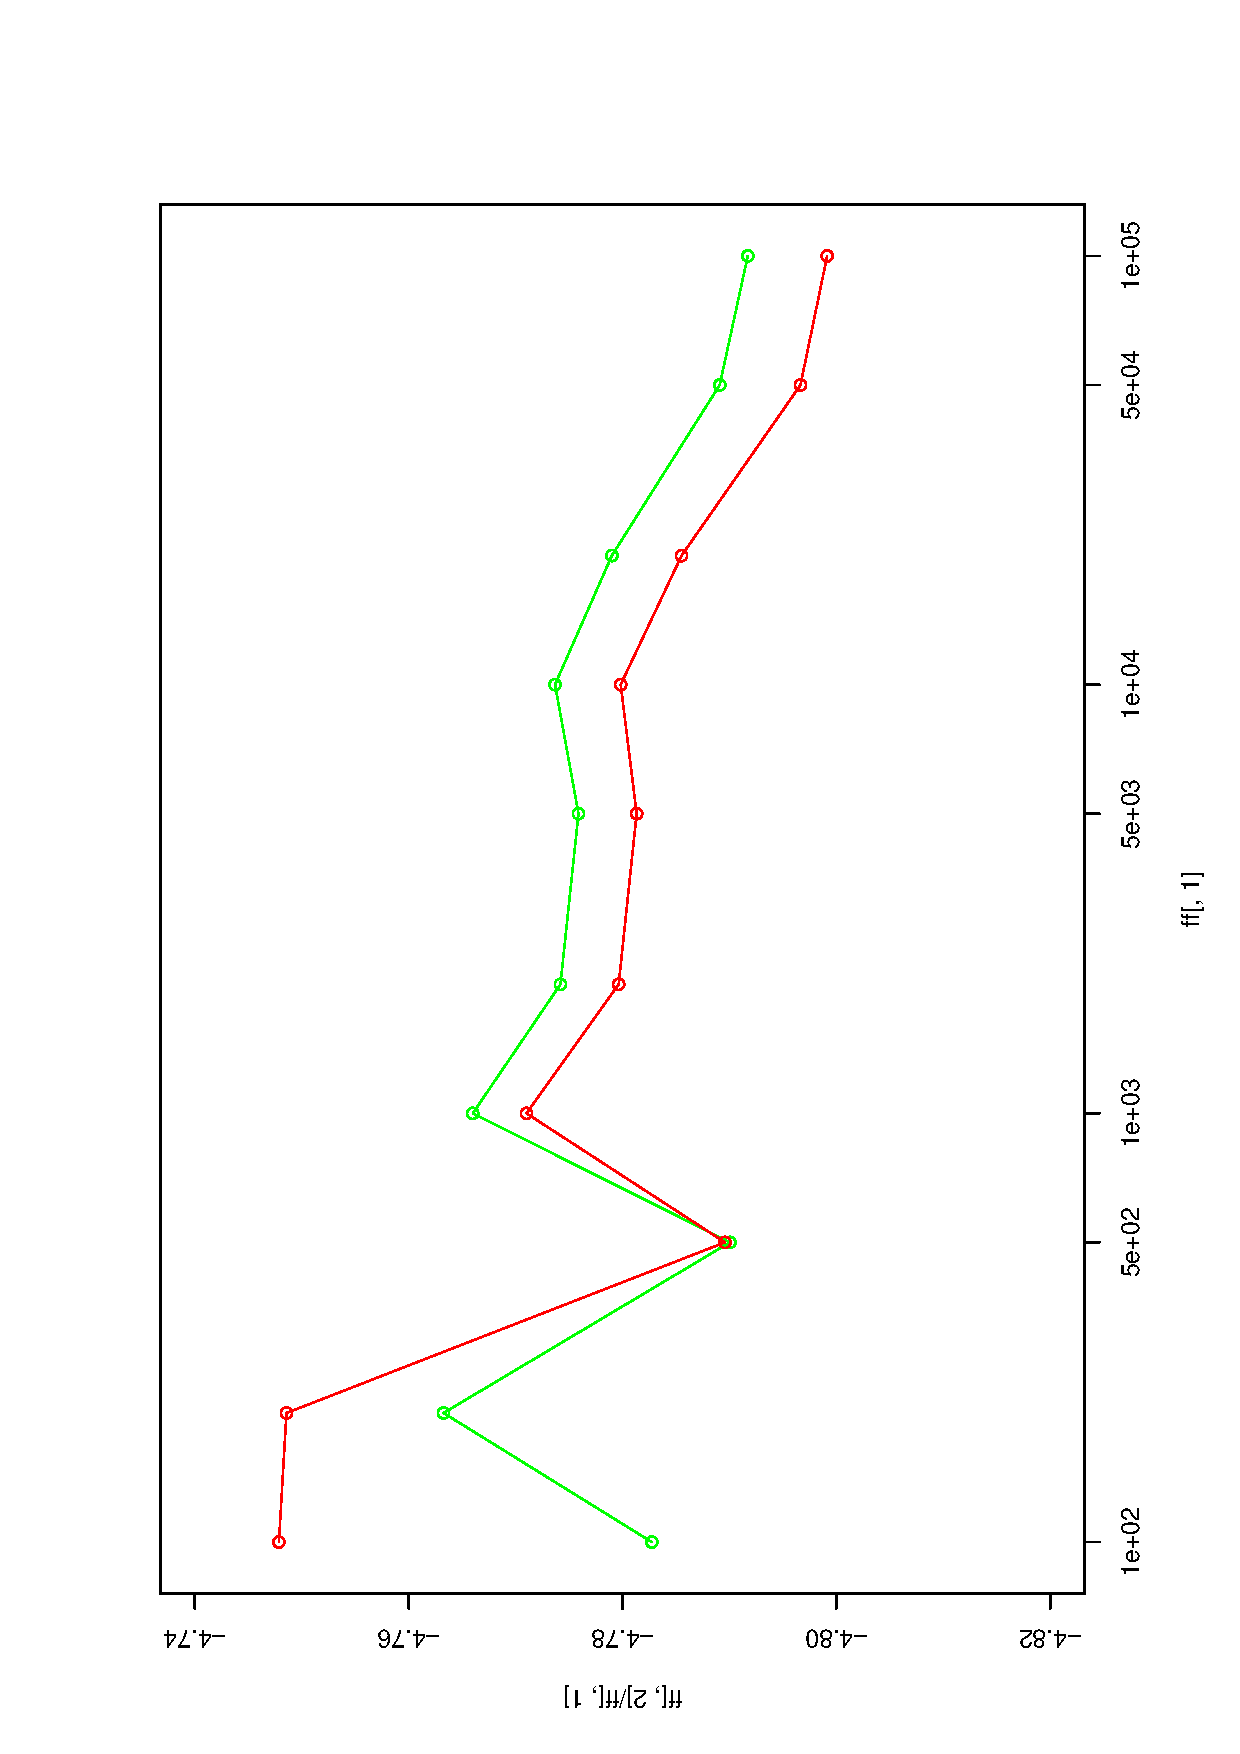
\includegraphics[width=3.0in]{loglpersite.idraw}}
\medskip

As more and more sites are added the true tree topology is favored.  Since
the vertical scale here is $\log(L)$ per site, the difference of log-likelihoods
becomes very great.

\end{slide}

\begin{slide}[Replace]{Rate variation among sites}
\medskip

Evolution is independent once each site has had its rate specified
\[
\begin{array}{l}
\mathsf{\Prob(D\; |\; T, r_1, r_2, \dots, r_p)\ = }\\
\\
\mathsf{~~~~\prod\limits_{i=1}^p \Prob(D^{(i)}\; |\; T, r_i)}.
\end{array}
\]

\end{slide}

\begin{slide}[Replace]{Coping with uncertainty about rates}
\medskip

Using a Gamma distribution independently assigning rates to sites:
\[
\mathsf{L\ =\ \prod_{i=1}^m \left[ \int_0^\infty f(r ; \alpha)\; L^{(i)}(r)\; dr \right]}
\]
Unfortunately this is hard to compute on a tree with more than a few species.

Yang (1994a) approximated this by a discrete histogram of rates:
\[
\mathsf{L^{(i)} \ =\ \int_0^\infty f(r ; \alpha)\; L^{(i)}(r)\; dr
\ \ \simeq\  \ \sum\limits_{j=1}^k w_k L^{(i)}(r_k)}
\]
Felsenstein (J. Mol. Evol., 2001) has suggested using Gauss-Laguerre quadrature to choose
the rates $~\mathsf{r_i}~$ and the weights $~\mathsf{w_i}$.

\end{slide}

\begin{slide}[Replace]{Hidden Markov Models}
\bigskip

These are the most widely used models allowing rate variation to be
correlated along the sequence.
\bigskip

We assume:
\begin{itemize}
\item There are a finite number of rates, $\mathsf{m}$.  Rate $i$ is $\mathsf{r_i}$.
\item There are probabilities $\mathsf{p_i}$ of a site having rate $\mathsf{i}$.
\item A process not visible to us (``hidden") assigns rates to
sites.  It is a Markov process working along the sequence.  For example
it might have transition probability $\mathsf{\Prob(j|i)}$ of changing to rate $\mathsf{j}$
in the next site, given that it is at rate $\mathsf{i}$ in this site.
\item The probability of our seeing some data are to be obtained by
summing over all possible combinations of rates, weighting appropriately
by their probabilities of occurrence.
\end{itemize}

\end{slide}

\begin{slide}[Replace]{Likelihood with a[n] HMM}
\bigskip

Suppose that we have a way of calculating, for each possible
rate at each possible site, the probability of the data at that
site $~\mathsf{(i)}~$ given that rate $~\mathsf{(r_j)}$.  This is

\[
\mathsf{\Prob\left(D^{(i)}\;|\;r_j\right)}
\]

This can be done because the probabilities of change as a function of
the rate $~\mathsf{r}~$ and time $~\mathsf{t}~$ are (in almost all
models) just functions of their product $~\mathsf{rt}$, so a site that
has twice the rate is just like a site that has branches twice as long.
\bigskip

To get the overall probability of all data, sum over all
possible paths through the array of sites $\mathsf{\times}$ rates,
weighting each combination of rates by its probability:

\end{slide}


\begin{slide}[Replace]{Hidden Markov Model of rate variation}

\centerline{\includegraphics[height=2.8in]{fig16-4.ydraw}}

\end{slide}

\begin{slide}[Replace]{Hidden Markov Models}
\bigskip

If there are a number of hidden rate states, with state $i$ having rate $r_i$
\[
\begin{array}{c c r}
\mathsf{\Prob(D\;|\;T)} & \mathsf{=} & \mathsf{\sum\limits_{i_1} \sum\limits_{i_2} \dots \sum\limits_{i_p} \Prob (r_{i_1}, r_{i_2}, \dots r_{i_p})}\\
\\
& & \mathsf{\times \ \Prob(D\;|\;T, r_{i_1}, r_{i_2}, \dots r_{i_m})}
\end{array}
\]
Evolution is independent once each site has had its rate specified
\[
\begin{array}{l}
\mathsf{\Prob(D\; |\; T, r_1, r_2, \dots, r_p)\ = }\\
\\
\mathsf{~~~~~~~\prod\limits_{i=1}^p \Prob(D^{(i)}\; |\; T, r_i)}.
\end{array}
\]

\end{slide}

\begin{slide}[Replace]{Seems impossible ...}
\bigskip

To compute the likelihood we sum over all ways rate states could be
assigned to sites:

\[
\renewcommand{\arraystretch}{2.0}
\begin{array}{c c l}
\mathsf{L} & \mathsf{=}  & \mathsf{\Prob(D\;|\;T)}\\
&  \mathsf{=} & \mathsf{\sum\limits_{i_1=1}^m \sum\limits_{i_2=1}^m \dots \sum\limits_{i_p=1}^m\ \Prob\left(r_{i_1}, r_{i_2}, \dots, r_{i_p}\right)} \\
& &\mathsf{\times\ \Prob\left(D^{(1)}\;|\;r_{i_1}\right) \Prob\left(D^{(2)}\;|\;r_{i_2}\right) \dots \Prob\left(D^{(n)}\;|\;r_{i_p}\right)}
\end{array}
\]
\bigskip

Problem: The number of rate combinations is very large.  With
100 sites and 3 rates at each, it is $\mathsf{3^{100} \simeq 5 \times 10^{47}}$.
This makes the summation impractical.

\end{slide}

\begin{slide}[Replace]{Factorization and the algorithm}
\bigskip

Fortunately, the terms can be reordered:
\[
\begin{array}{c c c l}
\mathsf{L}  & =  &   \mathsf{\Prob(D\;|\;T)}\\
& & \\
&  \mathsf{=} & \mathsf{\sum\limits_{i_1=1}^m\ \sum\limits_{i_2=1}^m\ \dots\ \sum\limits_{i_p=1}^m}
& \mathsf{\Prob(i_1)\ \Prob\left(D^{(1)}\;|\;r_{i_1}\right)}\\
& & &\mathsf{\times\ \Prob(i_2\;|\;i_1)\ \Prob\left(D^{(2)}\;|\;r_{i_2}\right)}\\
& & &\mathsf{\times\ \Prob(i_3\;|\;i_2)\ \Prob\left(D^{(3)}\;|\;r_{i_3}\right)}\\
& & &\\
& & &\mathsf{\vdots}\\
& & &\\
& & &\mathsf{\times\ \Prob(i_p\;|\;i_{p-1})\ \Prob\left(D^{(p)}\;|\;r_{i_p}\right)}
\end{array}
\]

\end{slide}

\begin{slide}[Replace]{Using Horner's Rule}
\bigskip

and the summations can be moved each as far rightwards as it
can go:
\[
\renewcommand{\arraystretch}{1.9}
\begin{array}{c c l}
\mathsf{L} & \mathsf{=}  & \mathsf{\sum\limits_{i_1=1}^m\ \Prob(i_1)\ \Prob\left(D^{(1)}\;|\;r_{i_1}\right)}\\
& & \raisebox{12pt}{\strut}\ \mathsf{\sum\limits_{i_2=1}^m\ \Prob(i_2\;|\;i_1)\ \Prob\left(D^{(2)}\;|\;r_{i_2}\right)}\\
& &\raisebox{12pt}{\strut} \ \ \mathsf{\sum\limits_{i_3=1}^m\ \Prob(i_3\;|\;i_2)\ \Prob\left(D^{(3)}\;|\;r_{i_3}\right)}\\
& &\ \ \ \ \mathsf{\vdots}\\
 & & \\
& & \ \ \ \ \mathsf{\sum\limits_{i_p=1}^m\ \Prob(i_p\;|\;i_{p-1})\ \Prob\left(D^{(p)}\;|\;r_{i_p}\right)}
\end{array}
\]

\end{slide}

\begin{slide}[Replace]{Recursive calculation of HMM likelihoods}
\bigskip

The summations can be evaluated innermost-outwards.  The same
summations appear in multiple terms.  We can then evaluate them
only once.  A huge saving results.  The result is this algorithm:

Define $\mathsf{{\cal P}_i(j)}$ as the probability of everything
at or to the right of site $\mathsf{i}$, given that site $\mathsf{i}$ has the
$\mathsf{j}$-th rate.

Now we can immediately see for the last site that for each possible
rate category $\mathsf{i_p}$
\[
\mathsf{{\cal P}_p(i_p)\ = \ \Prob\left(D^{(p)}\;|\;r_{i_p}\right)}
\]
(as ``at or to the right of" simply means ``at" for that site).

\end{slide}

\begin{slide}[Replace]{Recursive calculation}
\bigskip

More generally, for site $\mathsf{\ell < p}$ and its rates $\mathsf{i_\ell}$

\[
\mathsf{{\cal P}_\ell(i_\ell)\ \ = \ \ \Prob\left(D^{(\ell)}\;|\;r_{i_\ell}\right)
 \sum\limits_{i_\ell = 1}^m \ \Prob(i_{\ell+1}\;|\;i_\ell)\ {\cal P}_{\ell+1}(i_{\ell+1})}
\]

We can compute the $\mathsf{{\cal P}}$'s recursively using this,
starting with the last site and moving leftwards down the
sequence.  Finally we have the $\mathsf{{\cal P}_1(i_1)}$ for all $\mathsf{m}$
states.  These are simply weighted by the equilibrium
probabilities of the Markov chain of rate categories:
\[
\mathsf{L\ =\ \Prob(D\;|\;T)\ = \ \sum\limits_{i_1=1}^m\ \Prob(i_1)\ {\cal P}_1(i_1)}
\]
An entirely similar calculation can be done from left to right,
remembering that the transition probabilities $\mathsf{\Prob(i_k|i_{k+1})}$ would
be different in that case.

\end{slide}

% \begin{slide}[Replace]{Hidden Markov Models}
% \medskip
% 
% Summing over all combinations of rates, weighting by their prior
% probabilities:
% \[
% \begin{array}{c c l}
% \mathsf{\prob(D|T)} & \mathsf{=} & \mathsf{\sum\limits_{i_1} \sum\limits_{i_2}
% \dots \sum\limits_{i_m} \ \prob (r_{i_1}, r_{i_2}, \dots r_{i_m})}\\
% &  &\\
% & & \mathsf{\times  \prob(D | T, r_{i_1}, r_{i_2}, \dots r_{i_m})}
% \end{array}
% \]
% 
% There are too many possible combinations of rates.  How to economize on
% the computation?  One can use the ``backward algorithm" of HMM's:
% 
% First note that independence of evolution given the rate combination
% implies that
% \[
% \mathsf{\prob(D | T, r_1, r_2, \dots, r_m) \ = \ \prod\limits_{i=1}^m \prob(D^{(i)} | T, r_i)}
% \]
% We can precompute all the $\mathsf{\Prob(D^{(i)}\;|\;T, r_i)}$.
% 
% \end{slide}

\begin{slide}[Replace]{All paths through the array}

\centerline{\includegraphics[height=2.8in]{paths0.ydraw}}

\end{slide}

\begin{slide}[Replace]{Starting and finishing the calculation}

At the end, at site $\mathsf{m}$:
\[
\mathsf{\prob(D^{[m]} | T, r_{i_m})\ =\ \prob(D^{(m)} | T, r_{i_m})}
\]

and once we get to site 1, we need only use the prior probabilities of
the rates $\mathsf{r_i}$ to get a weighted sum:
\[
\mathsf{\prob(D | T) \ =\  \sum\limits_{i_1} \pi_{i_1} \prob(D^{[1]} | T, r_{i_1})}
\]

\end{slide}

\begin{slide}[Replace]{The pruning algorithm is just like}

\centerline{\includegraphics[width=2.9in]{prunehmm1.ydraw}}

\end{slide}

\begin{slide}[Replace]{the forward algorithm}

\centerline{\includegraphics[width=2.9in]{prunehmm2.ydraw}}

\end{slide}

\begin{slide}[Replace]{Paths from one state in one site}

\centerline{\includegraphics[height=2.8in]{paths1.ydraw}}

\end{slide}

\begin{slide}[Replace]{Paths from another state in that site}

\centerline{\includegraphics[height=2.8in]{paths2.ydraw}}

\end{slide}

\begin{slide}[Replace]{Paths from a third state}

\centerline{\includegraphics[height=2.8in]{paths3.ydraw}}

\end{slide}

\begin{slide}[Replace]{We can also use the backward algorithm}

\centerline{\includegraphics[height=2.8in]{paths4.ydraw}}

\end{slide}

\begin{slide}[Replace]{Using both we can find likelihood contributed by a state}

\centerline{\includegraphics[height=2.8in]{paths5.ydraw}}

\end{slide}

\begin{slide}[Replace]{A particular Markov process on rates}

There are many possible Markov processes that could be used in the HMM
rates problem.  I have used:
\[
\mathsf{\prob(r_i | r_j)\ =\ (1-\lambda)\; \delta_{ij} + \lambda\; \pi_i}
\]

\end{slide}

\begin{slide}[Replace]{A numerical example. Cytochrome B}

We analyze 31 cytochrome B sequences, aligned by Naoko Takezaki,
using the Proml protein maximum likelihood program.  Assume a
Hidden Markov Model with 3 states, rates:
\bigskip

\begin{center}
\begin{tabular}{c c c}
category & rate & probability \\
\hline
1 &  0.0 & 0.2 \\
2 & 1.0 & 0.4 \\
3 &  3.0 & 0.4
\end{tabular}
\end{center}
\bigskip


and expected block length  3.
\bigskip

We get a reasonable, but not perfect, tree with the best rate combination inferred
to be

\end{slide}

\begin{slide}[Replace]{Phylogeny for Takezaki cytochrome B}

\centerline{\includegraphics[width=3.5in]{cytb.ydraw}}

\end{slide}

\begin{slide}[Replace]{Rates inferred from Cytochrome B}

\noindent
~\hspace{-0.4in}{\ttfamily \ptsize{8}
\renewcommand{\arraystretch}{0.6}
\begin{tabular}{l l}
 &1333333311\ 3222322313\ 3321113222\ 2133111111\ 1331133123\ 1122111112 \\
\multicolumn{2}{c}{~}\\
african&M--------TPMR\ KINPLMKLIN\ HSFIDLPTPS\ NISAWWNFGS\ LLGACLILQI\ TTGLFLAMHYS\\
caucasian&..........\ .........R\ ..........\ ..........\ ..T.......\ ..........\\
cchimp&.......T..\ ..........\ ..........\ ..........\ ..........\ ..........\\
pchimp&.......T..\ ..........\ ..........\ ..T.......\ ..........\ ..........\\
gorilla1&..........\ T...A.....\ ..........\ ..T.......\ ..........\ ..........\\
gorilla2&..........\ T...A.....\ ..........\ ..T.......\ ..........\ ..........\\
borang&..........\ T.........\ .L........\ ..........\ ......I.TI\ ..........\\
sorang&......ST..\ T.........\ .L........\ ..........\ ......I...\ ..........\\
gibbon&.......L..\ T.........\ .L....A...\ ..M.......\ .........I\ .........T\\
bovine&......NI..\ SH....IV.N\ A.....A...\ ..S.......\ ..I......L\ .........T\\
whalebm&......NI..\ TH....I..D\ A.........\ ..S.......\ ..L...V..L\ .........T\\
whalebp&......NI..\ TH....IV.D\ A.V.......\ ..S.......\ ..L...M..L\ .........T\\
dhorse&......NI..\ SH..I.I...\ ......A...\ ..S.......\ ..I......L\ .........T\\
horse&......NI..\ SH..I.I...\ ..........\ ..S.......\ ..I......L\ .........T\\
rhinocer&......NI..\ SH..V.I...\ ..........\ ..S.......\ ..I......L\ .........T\\
cat&......NI..\ SH..I.I...\ ......A...\ ..........\ ..V..T...L\ .........T\\
gseal&......NI..\ TH....I..N\ ..........\ ..........\ ..I......L\ .........T\\
hseal&......NI..\ TH....I..N\ ..........\ ..........\ ..I......L\ .........T\\
mouse&......N...\ TH..F.I...\ ......A...\ ..S.......\ ..V..MV..I\ .........T\\
rat&......NI..\ SH..F.I...\ ......A...\ ..S.......\ ..V..MV..L\ .........T\\
platypus&.....NNL..\ TH..I.IV..\ ..........\ ..S.......\ ..L...I..L\ .........T\\
wallaroo&......NL..\ SH..I.IV..\ ......A...\ ..........\ ......I..L\ .........T\\
opossum&......NI..\ TH....I..D\ ..........\ ..........\ ..V...I..L\ .........T\\
chicken&....APNI..\ SH..L.M..N\ .L....A...\ ..........\ .AV..MT..L\ ...L.....T\\
xenopus&....APNI..\ SH..I.I..N\ ..........\ ..SL......\ ..V...A..I\ .........T\\
carp&....A-SL..\ TH..I.IA.D\ ALV.......\ ..........\ ..L...T..L\ .........T\\
loach&....A-SL..\ TH..I.IA.D\ ALV...A...\ ..V.......\ ..L...T..L\ .........T\\
trout&....A-NL..\ TH..L.IA.D\ ALV...A...\ ..V.......\ ..L..AT..L\ .........T\\
lamprey&.SHQPSII..\ TH..LS.G.S\ MLV...S.A.\ ..........\ .SL......I\ ...I.....T\\
seaurchin1&-...LG.L..\ EH.IFRIL.S\ T.V...L...\ L.I.......\ ..L...T..L\ .........T\\
seaurchin2&-...AG.L..\ EH.IFRIL.S\ T.V...L...\ L.M.......\ ..L...I.LI\ ..I......T\\
\end{tabular}
}

\end{slide}

\begin{slide}[Replace]{Rates inferred from Cytochrome B}

~\hspace{-0.4in}{\ttfamily \ptsize{8}
\renewcommand{\arraystretch}{0.6}
\begin{tabular}{l l}
&2223311112\ 2222222222\ 2222232112\ 2222222223\ 1222221112\ 3333111122\\
\multicolumn{2}{c}{~}\\
african&PDASTAFSSI\ AHITRDVNYG\ WIIRYLHANG\ ASMFFICLFL\ HIGRGLYYGS\ FLYSETWNIG\\
caucasian&..........\ ..........\ ..........\ ..........\ ..........\ ..........\\
cchimp&..........\ ..........\ ..........\ ..........\ ..........\ ...L......\\
pchimp&..........\ ..........\ ..........\ ...L......\ .V........\ ...L......\\
gorilla1&..........\ ..........\ .T........\ ..........\ ..........\ ..HQ......\\
gorilla2&..........\ ..........\ .T........\ ..........\ ..........\ ..HQ......\\
borang&...T......\ ..........\ .M..H.....\ ...L......\ ..........\ .THL......\\
sorang&..........\ ..........\ .M..H.....\ ..........\ ..........\ .THL......\\
gibbon&.........V\ ..........\ ..........\ ..........\ ..........\ ...L......\\
bovine&S.TT.....V\ T..C......\ .....M....\ ........YM\ .V........\ YTFL......\\
whalebm&..TM.....V\ T..C......\ .V........\ ........YA\ .M........\ HAFR......\\
whalebp&..TT.....V\ T..C......\ ..........\ ........YA\ .M........\ YAFR......\\
dhorse&S.TT.....V\ T..C......\ ..........\ .........I\ .V........\ YTFL......\\
horse&S.TT.....V\ T..C......\ ..........\ .........I\ .V........\ YTFL......\\
rhinocer&..TT.....V\ T..C......\ .M........\ .........I\ .V........\ YTFL......\\
cat&S.TM.....V\ T..C......\ ..........\ ........YM\ .V...M....\ YTF.......\\
gseal&S.TT.....V\ T..C......\ ..........\ ........YM\ .V........\ YTFT......\\
hseal&S.TT.....V\ T..C......\ ..........\ ........YM\ .V........\ YTFT......\\
mouse&S.TM.....V\ T..C......\ .L...M....\ ..........\ .V........\ YTFM......\\
rat&S.TM.....V\ T..C......\ .L....Q...\ ..........\ .V........\ YTFL......\\
platypus&S.T......V\ ...C......\ .L...M....\ ..L..M.I..\ ..........\ YTQT......\\
wallaroo&S.TL.....V\ ...C......\ .L..N.....\ .....M....\ .V...I....\ Y..K......\\
opossum&S.TL.....V\ ...C......\ .L..NI....\ .....M....\ .V...I....\ Y..K......\\
chicken&A.T.L....V\ ..TC.N.Q..\ .L..N.....\ ..F....I..\ ..........\ Y..K....T.\\
xenopus&A.T.M....V\ ...CF.....\ LL..N.....\ L.F....IY.\ ..........\ ...K......\\
carp&S.I......V\ T..C......\ .L..NV....\ ..F....IYM\ ..A.......\ Y..K......\\
loach&S.I......V\ ...C......\ .L..NI....\ ..F.....Y.\ ..A.......\ Y..K......\\
trout&S.I......V\ C..C...S..\ .L..NI....\ ..F....IYM\ ..A.......\ Y..K......\\
lamprey&ANTEL....V\ M..C....N.\ .LM.N.....\ .......IYA\ .....I....\ Y..K....V.\\
seaurchin1&A.I.L....A\ S..C......\ .LL.NV....\ ..L....MYC\ .........G\ SNKI....V.\\
seaurchin2&A.INL....V\ S..C......\ .LL.NV...C\ ..L....MYC\ .........L\ TNKI....V.\\
\end{tabular}
}

\end{slide}

\begin{slide}[Replace]{PhyloHMMs: used in the UCSC Genome Browser}

The conservation scores calculated in the Genome Browser use PhyloHMMs, which
is just these HMM methods.

\centerline{\includegraphics[width=4in]{phylohmm2.ps}}

\end{slide}

\end{document}
